\documentclass[a4paper, 10pt, twocolumn]{article}

\usepackage[resetfonts]{cmap}
\usepackage[english, czech]{babel}
\usepackage[utf8]{inputenc}
\usepackage[T1]{fontenc}
\usepackage{lmodern}

\usepackage{amsmath}
\usepackage{amssymb}
\usepackage{listings}
\usepackage{multicol}
\usepackage{graphicx}

\usepackage{hyperref}
\hypersetup{unicode=true}
\usepackage{microtype}

\title{WalkAuth\\
\large Závěrečná zpráva ze studentského projektu do předmětu PV021
}


\author{Čechák, Jaroslav\\
	\texttt{410322@mail.muni.cz}
	\and
	Effenberger, Tomáš\\
	\texttt{410350@mail.muni.cz}
	\and
	Mauritz, Jiří\\
	\texttt{409972@mail.muni.cz}
}
\date{}

\begin{document}
\twocolumn[\maketitle ]


\begin{abstract}
  Cílem tohoto projektu bylo vytvořit neuronovou síť schopnou porozumět údajům z~akcelerometru naměřeným během klasické chůze několika lidí. Naučili jsme neuronovou síť rozpoznávat jednoho z~nich a na dalších vzorcích jsme zjišťovali, zda je možné ho odlišit od ostatních jen podle stylu chůze. Strukturu vstupních dat, neuronovou síť a proces učení jsme navrhli co nejvíce obecné a konfigurovatelné, abychom mohli pozorovat důsledky změny parametrů na výslednou úspěšnost. Použili jsme klasickou vícevrstvou neuronovou síť a učení s~učitelem aplikujeme pomocí gradientního sestupu a zpětné propagace.
\end{abstract}

\section{Zpracování dat}
    \subsection{Formát dat}
        Data byla stažena ze zdrojů online repozitáře UCI Machine Learning Repository \footnote{\url{http://archive.ics.uci.edu/ml/datasets/User+Identification+From+Walking+Activity}}. Dataset se jmenuje \textit{User Identification From Walking Activity Data Set}  a je strukturován do 22 csv souborů, kde každý soubor představuje chůzi jednoho uživatele. Každý záznam z~akcelerometru obsahuje čas měření a derivaci pohybu v~každém ze tří směrů x,y,z. Časy měření nejsou synchronizované, ale jsou závislé na rychlosti zápisu akcelerometru. Úlohu jsme si zjednodušili tím, že jsme ignorovali čas měření, protože všichni používali stejný akcelerometr, a tedy stejný počet záznamů odpovídal přibližně stejnému počtu milisekund v~každém záznamu. Čas chůze je různý pro jednotlivé uživatele a pohybuje se od 30 sekund do 11 minut.
    \subsection{Rozdělení dat}\label{rozdeleni_dat}
        Jeden vzorek (v~dokumentaci označovaný jako sample) odpovídá určitému počtu záznamů, který lze určit parametrem. Výchozí hodnota je 100 záznamů, což odpovídá přibližně třem sekundám chůze. Takový vzor následně slouží jako jeden vstup do neuronové sítě. Protože je jeden záznam složen ze tří číselných hodnot, vstup do neuronové sítě je třikrát větší, než je počet záznamů v~jednom vzorku.
        Rozhodli jsme se rozdělit data na tři množiny: trénovací, testovací a validační. Rozdělení dat mezi tyto množiny je možné upravit pomocí parametrů, ale výchozí hodnoty jsou trénovací 70\%, testovací 20\% a validační 10\%. Trénovací data používáme pro učení sítě, testovací použijeme na závěr učení pro otestování úspěšnosti naučené sítě a validační množina slouží ke kontrole přeučení. Rozdělení vzorků do těchto tří množin je v~každém procesu učení náhodné. Výskyt pozitivních a negativních vzorků je rovnoměrný pro všechny tři množiny.

    \subsection{Normalizace dat}
        Všechny tři množiny jsme normalizovali podle střední hodnoty a směrodatné odchylky naměřené v~trénovacích datech. Takto jsme nezavedli žádnou informaci o~testovacích datech do trénovací množiny. Normalizovali jsme data na střední hodnotu 0 a směrodatnou odchylku 1. Původní data mají střední hodnotu $2,26$ a směrodatnou odchylku $5,57$.
\section{Popis implementace}
    Projekt jsme implementovali v~jazyce Java.
    Zpracování dat pro neuronovou síť zajišťuje třída \texttt{DataManager} (přičemž normalizaci deleguje na třídu \texttt{Normalization} a jeden vzorek je reprezentován třídou \texttt{Sample}).
    Pro reprezentaci neuronové sítě (její topologie a vah) slouží třída \texttt{NeuralNetwork}. Tato třída umožňuje také provádět dopředný výpočet pro zadaný vstupní vzorek.
    Učení neuronové sítě pak zajišťuje třída \texttt{NeuralNetoworkLearning}. Proces učení začíná nastavením náhodných počátečních vah (popsané podrobněji níže), po kterém následuje klasický gradientní sestup využívající zpětné propagace pro výpočet gradientu čtvercové chyby vzhledem k~hodnotám vah.
    Třída \texttt{Evaluation} implementuje všechny použité evaluační metriky (čtvercová chyba, RMSE, precision, recall a F1).
    Dále už projekt obsahuje pouze několik pomocných tříd, např. pro práci s~maticemi, výpočet aktivační funkce (hyperbolický tangens) a její derivace a logování.
    Většina funkcionality našeho projektu je pokrytá jednotkovými testy.
    V~následujících odstavcích popisujeme některé zajímavé detaily.

    \subsection{Inicializace vah}
      Počáteční váhy jsme nastavili náhodně v~intervalu $[-w,w]$, kde $w$ je hodnota společná pro váhy vstupující do stejné vrstvy v~neuronové síti. Hodnotu $w$ jsme spočítali $w = \sqrt{\frac{3}{d}}$ kde $d$ je počet vstupů do jednoho neuronu vyšší vrstvy. Takto váhy do neuronu s~vyšším počtem vstupů byly menší než váhy do neuronu s~méně vstupy, a proto jejich potenciál byl srovnatelný na počátku učení. Vycházeli jsme z~doporučení v~materiálech předmětu PV021.

    \subsection{Test zpětné propagace}
    Jedním z~klíčových algoritmů našeho projektu je zpětná propagace.
    Rozhodli jsme se ho pořádně otestovat jednotkovými testy, ručně však bylo možné připravit pouze extrémně triviální případy.
    Proto jsme implementovaly jednoduchý numerický výpočet zpětné propagace a pak napsali řadu testů, které kontrolují, že pro různé topologie, aktuální nastavení vah a trénovací data vracejí numerický výpočet gradientu a zpětná propagace stejné výsledky (až na malou odchylku).
    Numerický výpočet gradientu funguje následovně: pro každou váhu $i$ spočítáme pro dostatečně malé $\delta$ gradient vzhledem k~této váze zvlášť numericky pomocí vzorce
    $$\frac{E(\ldots, \theta_i + \delta, \ldots) - E(\ldots, \theta_i - \delta, \ldots)}{2\delta}$$
    kde $E$ je čtvercová chyba pro dané nastavení vah.
    Takový výpočet gradientu je sice neefektivní (takže ho nelze použít při učení), zato však velmi jednoduchý na implementaci a mnohem méně náchylný na chyby než algoritmus zpětné propagace.
    Pořádné otestování zpětné propagace se vyplatilo, protože v~prvotní implementaci bylo hned několik chyb, které jsme díky testům okamžitě odhalili a mohli odladit ještě před zapojením funkce do gradientního sestupu.


\section{Výsledky a parametry}
Každý běh programu a učení neuronové sítě je náhodné jednak díky inicializaci vah, ale zejména kvůli náhodnému rozdělení vzorků na trénovací, validační a testovací část (viz \ref{rozdeleni_dat}). Průměrně však neuronová síť dosahuje s~výchozími parametry $\approx 75\% $ úspěšnosti rozpoznání naučeného člověka. Nejhorší pozorovaná úspěšnost s~výchozími parametry byla $69~\%$ a naopak nejlepší $83~\%$. Ve výchozí konfiguraci se učí síť typu 300-30-1 po dobu 400 iterací. Základ pro výpočet rychlosti učení je hodnota 0.005, která je v~každém kroku vynásobena aktuální chybou sítě na trénovacích datech a podělena počtem proběhlých iterací. Celkově se rychlost učení postupně snižuje a učení konverguje k~nějaké konečné hodnotě vah. Zkoušeli jsme různé kombinace parametrů a tyto se ukázaly jako nejlepší. Pro lepší vizualizaci a pochopení výsledků učení nám posloužily grafy rozložení naučených vah skryté vrstvy. Příklad jednoho takového je vidět níže na obrázku \ref{weighs}. Sloupce reprezentují jednotlivé skryté neurony a každý neuron je rozdělen na tři sloupce vah (osy měřeného zrychlení). Barva pak udává hodnotu váhy neuronu.  

\begin{figure}[ht]
\centering
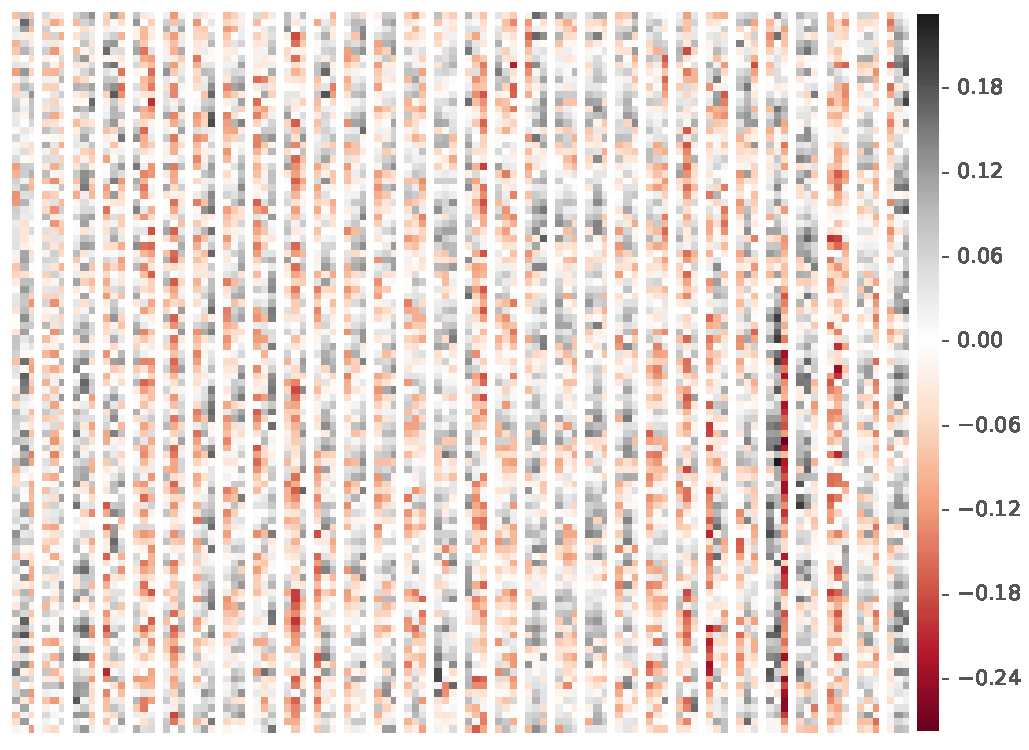
\includegraphics[width=0.5\textwidth]{img/weights.pdf}
\caption{Výsledné hodnoty váh skrýté vrstvy naučené neuronové sítě.}
\label{weighs}
\end{figure}


Ačkoli je značně obtížné přesně interpretovat chování neuronové sítě, v~obrázku si lze všimnout jistých ,,vzorů``. Jsou vidět posloupnosti extrémů vah, kdy se neuron zaměřil na zrychlení v~jednom ze směrů. Druhým vzorem jsou pak ,,vlny`` stejných vah napříč neurony, což interpretujeme jako snahu odhalit různou rychlost chůze.
\section{Diskuse}
    Výsledky ukazují průměrnou úspěšnost sítě kolem 75 \%, která hodně kolísá v~závislosti na rozdělení vzorků a inicializaci vah mezi 70 \% a 80 \%. Celkově výsledky nejsou uspokojivé natolik, aby mohla být síť použita v~reálné aplikaci. Našli jsme hned několik důvodů, proč si myslíme, že se tak stalo. První příčina je nedostatek dat, protože i pro určování uživatele s~nejdelší chůzí jsme pracovali s~celkovým počtem 300 vzorků. Snížením počtu záznamů na vzorek jsme mohli získat větší množinou vzorků, ale síť špatně rozpoznávala vstupy s~méně než třemi sekundami chůze. Dále s~tím souvisí i nízká úspěšnost při rozpoznávání dalších uživatelů s~málo vstupy (krátkou chůzí). Pro některé z~nich se síť učila pouze na desítkách vzorků, což nestačilo na naučení.
    \paragraph{}
    Dalším problémem mohlo být různé načasování vzorků chůze. Protože v~datech není žádná informace o~krocích, rozdělili jsme data jen podle počtu záznamů. Některé vzorky tak mohou začínat došlapem uživatele levou nohou a jiné jejím zvedáním. Předpokládáme, že dobrá neuronová síť si s~takovými nepřesnostmi poradí, ale v~našem případě nemáme analýzu na potvrzení, zda tomu tak u~naší sítě opravdu je.
    \paragraph{}
    Pokud by naše neuronová síť dosahovala vyšší úspěšnosti, bylo by možné ji využít jako autentizační mechanismus v~mobilních zařízeních. Použití by bylo následovné: uživatel naučí aplikaci svou chůzi na několika vzorcích v~různých terénech a aplikace bude následně kontrolovat, zda chůze odpovídá naměřené. Pokud zjistí, že se chůze liší, může jít o~krádež a aplikace zareaguje zablokováním, sms zprávou nebo dalšími způsoby.
    
\appendix
\section{Návod na použití}
Pro spuštění aplikace je potřeba mít nainstalované \textbf{JRE 1.8}. Starší verze Javy fungovat nebudou. Samotná aplikace se pak spouští z~příkazové řádky příkazem \texttt{java -jar WalkAuth.jar}. Pro zobrazení nápovědy stačí přidat standardně přepínač \texttt{-h} na konec příkazu. Aplikace dovoluje přenastavit parametry učení skrze přepínače. Všechny dostupné volby jsou uvedeny v~nápovědě včetně stručného popisku. Zdrojové kódy aplikace jsou veřejně dostupné elektronicky na adrese \url{https://github.com/jirmauritz/WalkAuth}.

\section{Rozdělení práce}
\paragraph{Jiří Mauritz}
\begin{itemize}
  \item získání, analýza dat
  \item rozdělení a normalizace dat
  \item implementace iniciálního nastavení vah neuronové sítě
  \item nastavení parametrů a jejich ladění
\end{itemize}


\paragraph{Jaroslav Čechák}
\begin{itemize}
\item implementace neuronové sítě a jejího dopředného výpočtu
\item implementace gradientního sestupu (mimo výpočet samotného gradientu)
\item ladění parametrů
\item CLI a finální infrastruktura pro snadné používání aplikace
\end{itemize}


\end{document}
